
\begin{figure}
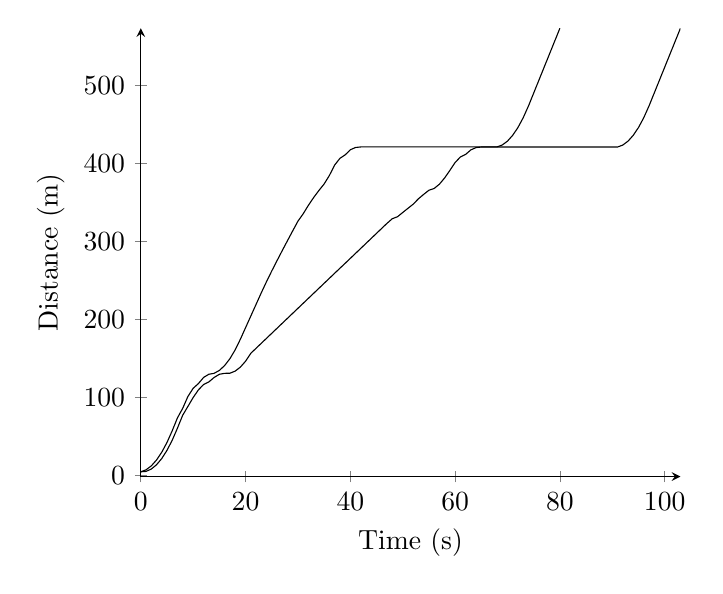
\begin{tikzpicture}
\begin{axis}[
legend style={anchor=west},
axis x line=bottom,
axis y line=left,
ymin=-1,
xlabel=Time (s),
ylabel=Distance (m),
]
\addplot[] coordinates {
(0, 5.1)
(1, 7.6)
(2, 12.6)
(3, 20.1)
(4, 30.1)
(5, 42.6)
(6, 57.6)
(7, 74.2)
(8, 86.34)
(9, 101.632252112)
(10, 112.059454389)
(11, 118.089689106)
(12, 126.079818867)
(13, 130.071924431)
(14, 131.27865093)
(15, 134.985377429)
(16, 141.192103928)
(17, 149.898830427)
(18, 161.105556926)
(19, 174.812283425)
(20, 189.716016757)
(21, 204.616203259)
(22, 219.516454659)
(23, 234.416786067)
(24, 248.719796798)
(25, 262.415614215)
(26, 275.568116012)
(27, 288.5078166)
(28, 301.229979021)
(29, 313.802459094)
(30, 326.272731973)
(31, 335.674001473)
(32, 346.656674161)
(33, 356.548357021)
(34, 365.557201236)
(35, 373.928577394)
(36, 384.799953552)
(37, 398.090380125)
(38, 406.672404625)
(39, 411.143848866)
(40, 417.756295639)
(41, 420.685150679)
(42, 421.361840866)
(43, 421.399879422)
(44, 421.399879422)
(45, 421.399879422)
(46, 421.399879422)
(47, 421.399879422)
(48, 421.399879422)
(49, 421.399879422)
(50, 421.399879422)
(51, 421.399879422)
(52, 421.399879422)
(53, 421.399879422)
(54, 421.399879422)
(55, 421.399879422)
(56, 421.399879422)
(57, 421.399879422)
(58, 421.399879422)
(59, 421.399879422)
(60, 421.399879422)
(61, 421.399879422)
(62, 421.399879422)
(63, 421.399879422)
(64, 421.399879422)
(65, 421.399879422)
(66, 421.399879422)
(67, 421.399879422)
(68, 421.399879422)
(69, 423.899879422)
(70, 428.899879422)
(71, 436.399879422)
(72, 446.399879422)
(73, 458.899879422)
(74, 473.899879422)
(75, 490.499879422)
(76, 507.099879422)
(77, 523.699879422)
(78, 540.299879422)
(79, 556.899879422)
(80, 573.499879422)
};
\addplot[] coordinates {
(0, 5.1)
(1, 5.58074069841)
(2, 8.56148139682)
(3, 14.0422220952)
(4, 22.0229627936)
(5, 32.503703492)
(6, 45.4844441904)
(7, 60.9651848889)
(8, 77.5651848889)
(9, 88.8429863738)
(10, 100.259155854)
(11, 110.023651985)
(12, 117.029657374)
(13, 120.253762291)
(14, 125.977867207)
(15, 130.031005698)
(16, 131.271719173)
(17, 131.398657228)
(18, 134.025595282)
(19, 139.152533337)
(20, 146.779471392)
(21, 156.906409447)
(22, 163.315649462)
(23, 169.724928975)
(24, 176.134251059)
(25, 182.543619113)
(26, 188.953036908)
(27, 195.362508637)
(28, 201.772038983)
(29, 208.181633182)
(30, 214.591297116)
(31, 221.001037413)
(32, 227.410861566)
(33, 233.820778083)
(34, 240.230796665)
(35, 246.640928419)
(36, 253.051186125)
(37, 259.461584565)
(38, 265.872140928)
(39, 272.18287532)
(40, 278.596882619)
(41, 285.010951629)
(42, 291.425091356)
(43, 297.839312651)
(44, 304.253628701)
(45, 310.668055706)
(46, 317.082613778)
(47, 323.497328214)
(48, 329.365475544)
(49, 331.938479211)
(50, 337.364801448)
(51, 342.720478717)
(52, 348.042787956)
(53, 354.962961705)
(54, 360.587251102)
(55, 365.901756627)
(56, 368.148317213)
(57, 373.651905174)
(58, 381.655493136)
(59, 391.281922138)
(60, 401.388409316)
(61, 408.488756189)
(62, 411.784719062)
(63, 417.580681934)
(64, 420.546830315)
(65, 421.239963828)
(66, 421.279867309)
(67, 421.279867309)
(68, 421.279867309)
(69, 421.279867309)
(70, 421.279867309)
(71, 421.279867309)
(72, 421.279867309)
(73, 421.279867309)
(74, 421.279867309)
(75, 421.279867309)
(76, 421.279867309)
(77, 421.279867309)
(78, 421.279867309)
(79, 421.279867309)
(80, 421.279867309)
(81, 421.279867309)
(82, 421.279867309)
(83, 421.279867309)
(84, 421.279867309)
(85, 421.279867309)
(86, 421.279867309)
(87, 421.279867309)
(88, 421.279867309)
(89, 421.279867309)
(90, 421.279867309)
(91, 421.279867309)
(92, 423.779867309)
(93, 428.779867309)
(94, 436.279867309)
(95, 446.279867309)
(96, 458.779867309)
(97, 473.779867309)
(98, 490.379867309)
(99, 506.979867309)
(100, 523.579867309)
(101, 540.179867309)
(102, 556.779867309)
(103, 573.379867309)
};

\end{axis}
\end{tikzpicture}
\label{tik:100:88}
\caption{100 percent diving with GSC on route $88$}
\end{figure}
